\documentclass[12pt, a4paper, oneside]{Thesis} 
% Paper size, default font size and one-sided paper
% \usepackage{biblatex}

\usepackage{wrapfig}
\usepackage{lscape}
\usepackage{rotating}
\usepackage{graphicx}
\usepackage{caption}
\usepackage{amsmath}
\usepackage[export]{adjustbox}

\usepackage{lineno,hyperref}
\modulolinenumbers[5]
\usepackage{xcolor}
\usepackage[export]{adjustbox}
\usepackage{amssymb}
\usepackage{graphicx}
\usepackage{array}
\usepackage{float}
\usepackage{placeins}
\usepackage{stackengine}
\usepackage{url}
\usepackage{numprint}
\usepackage{caption}

\usepackage{booktabs}  
\usepackage{siunitx}
\nprounddigits{3}
\newcolumntype{P}[1]{>{\centering\arraybackslash}p{#1}}
\newcolumntype{M}[1]{>{\centering\arraybackslash}m{#1}}

\setstackEOL{\#}
\setstackgap{L}{12pt}
\graphicspath{{Pictures/}} % Specifies the directory where pictures are stored
\usepackage{natbib}

\hypersetup{urlcolor=black, colorlinks=false} % Colors hyperlinks in blue - change to black if annoyingv`	

\thesistitle{Automatic Detection of Keyframe and Motion frame in Bharatanatyam Video}
\supervisor{Professor Partha Pratim Das}
\degree{Master of Technology}
\degreemajor{Computer Science and Engineering}
\authors{Heeramani Prasad (15CS30015)}
\university{Indian Institute of Technology Kharagpur}
\department{Department of Computer Science and Engineering}
\unisite{http://www.iitkgp.ac.in}
\depsite{http://www.cse.iitkgp.ac.in/}
\placeshrt{Kharagpur}
\placelng{Kharagpur - 721302, India}
\datesub{May 03, 2020}
\datesig{May 03, 2020}
\semsub{Spring Semester, 2019-20}
\coursecd{Master Thesis Project }

\title{\ttitle} % Defines the thesis title - don't touch this
\begin{document}
%\makeatletter
%\renewcommand*{\NAT@nmfmt}[1]{\textsc{#1}}
%\makeatother

% prints author names as small caps


\frontmatter % Use roman page numbering style (i, ii, iii, iv...) for the pre-content pages

\setstretch{1.6} % Line spacing of 1.6 (double line spacing)

% Define the page headers using the FancyHdr package and set up for one-sided printing
\fancyhead{} % Clears all page headers and footers
\rhead{\thepage} % Sets the right side header to show the page number
\lhead{} % Clears the left side page header

%\pagestyle{fancy} % Finally, use the "fancy" page style to implement the FancyHdr headers

\newcommand{\HRule}{\rule{\linewidth}{0.5mm}} % New command to make the lines in the title page

% PDF meta-data
\hypersetup{pdftitle={\ttitle}}
\hypersetup{pdfsubject=\subjectname}
\hypersetup{pdfauthor=\authornames}
\hypersetup{pdfkeywords=\keywordnames}

%----------------------------------------------------------------------------------------
%	TITLE PAGE
%----------------------------------------------------------------------------------------
\maketitle
%\titlepg % Add a gap in the Contents, for aesthetics

\clearpage % Start a new page

%----------------------------------------------------------------------------------------
%	DECLARATION PAGE
%	Your institution may give you a different text to place here
%----------------------------------------------------------------------------------------


% \Declaration% Add a gap in the Contents, for aesthetics


%----------------------------------------------------------------------------------------
%	CERTIFICATE PAGE
%----------------------------------------------------------------------------------------

\addtotoc{Certificate} % Add the "Abstract" page entry to the Contents

\certificate{\addtocontents{toc}{} % Add a gap in the Contents, for aesthetics

\clearpage % Start a new page

%----------------------------------------------------------------------------------------
%	ABSTRACT PAGE
%----------------------------------------------------------------------------------------

% \addtotoc{Abstract} % Add the "Abstract" page entry to the Contents

% \abstract{\addtocontents{toc}{} % Add a gap in the Contents, for aesthetics


% }

% \clearpage % Start a new page



%----------------------------------------------------------------------------------------
%	ACKNOWLEDGEMENTS
%----------------------------------------------------------------------------------------

\setstretch{1.3} % Reset the line-spacing to 1.3 for body text (if it has changed)

\acknowledgements{\addtocontents{toc}{}%\vspace{1em}} % Add a gap in the Contents, for aesthetics

We want to express our sincere gratitude to our Master Thesis Project guide professor Partha Pratim Das for the constant support for our study and related research, for his persistence, motivation, and extensive experience. His supervision helped in all the time of research and authorship of this report. We could not have believed having a better advisor and guide. Besides our guide, We would like to thank PhD student Mr.Himadri B.G.S. Bhuyan for his insightful comments and assistance to widen our research from various viewpoints.

Thank you.
}
\clearpage % Start a new page

%----------------------------------------------------------------------------------------
%	LIST OF CONTENTS/FIGURES/TABLES PAGES
%----------------------------------------------------------------------------------------

\pagestyle{fancy} % The page style headers have been "empty" all this time, now use the "fancy" headers as defined before to bring them back

\lhead{\emph{Contents}} % Set the left side page header to "Contents"
\tableofcontents % Write out the Table of Contents

\lhead{\emph{List of Figures}} % Set the left side page header to "List of Figures"
\listoffigures % Write out the List of Figures

\lhead{\emph{List of Tables}} % Set the left side page header to "List of Tables"
\listoftables % Write out the List of Tables

%----------------------------------------------------------------------------------------
%	ABBREVIATIONS
%----------------------------------------------------------------------------------------

\clearpage % Start a new page

\setstretch{1.5} % Set the line spacing to 1.5, this makes the following tables easier to read

\lhead{\emph{Abbreviations}} % Set the left side page header to "Abbreviations"
\listofsymbols{ll} % Include a list of Abbreviations (a table of two columns)
{
\textbf{KF} & \textbf{K}ey \textbf{F}rame \\
\textbf{MF} & \textbf{M}otion \textbf{F}rame \\
\textbf{KP} & \textbf{K}ey \textbf{P}ostures \\
\textbf{ICD} & \textbf{I}ndian \textbf{C}lassical \textbf{D}ance \\
\textbf{HOOF} & \textbf{H}istogram \textbf{O}f \textbf{O}ptical \textbf{F}low \\
\textbf{SVM} & \textbf{S}upport \textbf{V}ector \textbf{M}achine \\
\textbf{OF} & \textbf{O}ptical \textbf{F}low \\
\textbf{LK} & \textbf{L}ucas \textbf{K}anade \\
\textbf{TP} & \textbf{T}rue \textbf{P}ositive \\
\textbf{TN} & \textbf{T}rue \textbf{N}egative \\
\textbf{FP} & \textbf{F}alse \textbf{P}ositive \\
\textbf{FN} & \textbf{F}alse \textbf{N}egative \\
\textbf{ACC} & \textbf{A}ccuracy \\
\textbf{Min} & \textbf{M}inimum \\
\textbf{Max} & \textbf{M}aximum \\
\textbf{\%age} & \textbf{P}ercentage \\
\textbf{hist} & \textbf{H}istogram \\
\textbf{RGB} & \textbf{R}ed \textbf{G}reen \textbf{B}lue\\
\textbf{fps} & \textbf{F}rame \textbf{P}er \textbf{S}econd\\
}

%----------------------------------------------------------------------------------------
%	DEDICATION
%----------------------------------------------------------------------------------------
%
%\setstretch{1.3} % Return the line spacing back to 1.3
%
%\pagestyle{empty} % Page style needs to be empty for this page
%
%\dedicatory{For/Dedicated to/To my\ldots} % Dedication text
%
%\addtocontents{toc}{\vspace{2em}} % Add a gap in the Contents, for aesthetics

%----------------------------------------------------------------------------------------
%	THESIS CONTENT - CHAPTERS
%----------------------------------------------------------------------------------------

\mainmatter % Begin numeric (1,2,3...) page numbering

\pagestyle{fancy} % Return the page headers back to the "fancy" style

% Include the chapters of the thesis as separate files from the Chapters folder



\chapter{Introduction} % Main chapter title

\label{Chapter 1} 
\lhead{Chapter 1. \emph{Introduction}} 


There are following eight forms of dance recognized by the Sangeet Natak Akademi \citep{wiki:004}.

\begin{enumerate}
    \item Bharatanatyam
    \item Kathakali
    \item Odissi
    \item Kathak
    \item Kuchipudi
    \item Mohiniyattam
    \item Manipuri
    \item Sattriya
\end{enumerate}

These all dance types represent South Indian religious texts and religious beliefs, especially of Shaivism, Vaishnavism and Shaktism. \citep{williams2004shadow}

Bharatanatyam is a important form of IDC (Indian classical dance) that began in the state of Tamil Nadu hundreds of years ago. \citep{williams2004shadow}. Its origin can be traced back to the Natya Sastra. It is a Sanskrit text written by sage Bharata Muni on the performing arts. Bharatnatyam  was originated of two words, ‘Bharata’ and ’Natyam’, where 'Bharata' is a mnemonic containing ‘bha’, ‘ra’ and ‘ta’ which respectively.
Here ‘bhava’ is emotion and feelings; ‘raga’ is a melody, and ‘tala’ beats.
In Hindus temples, Bharatanatyam was exclusive up to the $19^th$ century. In modern days, Bharatanatyam spread out to different parts of India and available on the internet easily.
 
 Bharatanatyam dance movements are portrayed by bent legs, while feet keep beat. In a set of mudras, symbolic hand gestures are used to express a story.
 
 Bharatanatyam have basic choreographic units of a dance sequence. An Adavu is accompanied by percussion and vocal music and follows a specific rhythmic pattern \citep{mallick2018characterization}.

 \begin{figure}
    \centering
    \subfigure[]{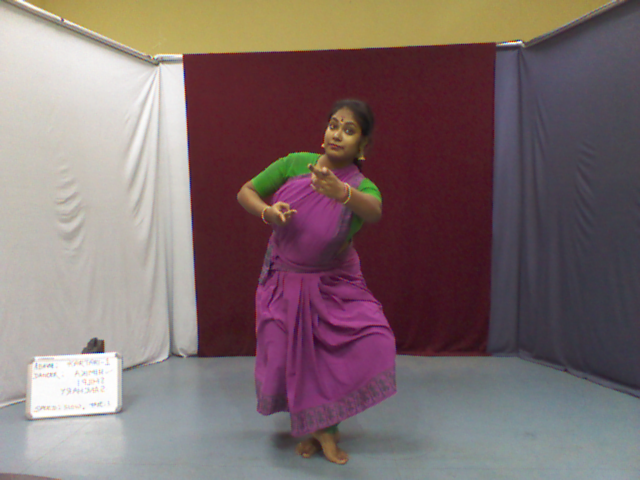
\includegraphics[width=0.32\textwidth]{Pictures/color_USB-VID_045E&PID_02BF-0000000000000000_239.png}} 
    \subfigure[]{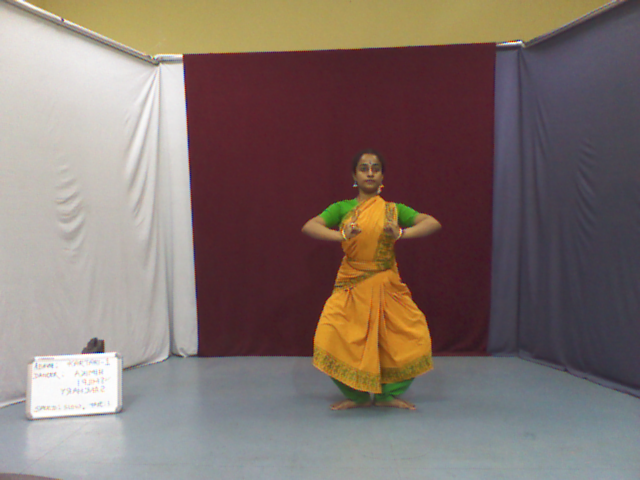
\includegraphics[width=0.32\textwidth]{Pictures/color_USB-VID_045E&PID_02BF-0000000000000000_74.png}} 
    \subfigure[]{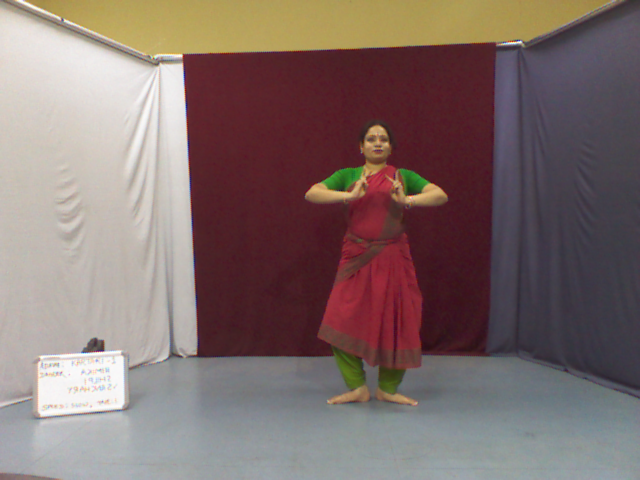
\includegraphics[width=0.32\textwidth]{Pictures/color_USB-VID_045E&PID_02BF-0000000000000000_14.png}}
    \caption{(a) Dancer 1 (b) Dancer 2 (c) Dancer 3}
    \caption{Bharatanatyam, Katti kartari Adavu, Variation 1}
    \label{fig:Ch01001}
\end{figure}

There are following classification of Adavus in Bharatnatyam. There are multiple variations under Adavus in Bharatnatyam.
\begin{enumerate}
    \item Tattu Adavu
    \item Nattu Adavu
    \item Pakka Adavu
    \item Kudditu Mettu Adavu
    \item Kudditu Nattal Adavu
    \item Kudditu Tattal Adavu
    \item Paikal Adavu
    \item Tei Tei Dhatta
    \item Katti Kartari as shown in Figure \ref{fig:Ch01001}
    \item Utsanga Adavu
    \item Mandi Adavu
    \item Sarrikkal Adavu
    \item Tirmana Adavu
    \item Sarika Adavu
    \item Joining Adavu
\end{enumerate}

\section{Bharatnatyam \& Computer Vision}
Bharatnatyam contains a large number of motion frames and Key Postures.

In Computer Vision, Human motion, representation and  its characteristic is an important topic. They are represented and displayed in various forms through centuries.
Human identification using motion analysis is mainly focused on observing human gait.
The motion of a person's legs and motion of a person's arms are considered as human gait.
There is motion information available in dance frames of Adavus. So, 
a high-level feature representation of the dance frame has used using Histogram of optical flow (HOOF).

There are following dancers as shown in Figure \ref{fig:Ch01001}, for Katti Kartari Adavu in Variation 1.


 


Following important terminology are associated with \textbf{Bharatanatyam Dance}:
\begin{itemize}
    \item \textbf{Adavu:} The basic unit of Bharatanatyam.
    \item \textbf{Key Postures(KP):} Momentarily stationary well-defined postures occur within the Adavu
    \item \textbf{Key Frames(KF):} Frames associated with a Key Posture
    \item \textbf{Motion Frames(MF):} Frames associated with motion
\end{itemize}

\section{Introduction to Keyframe and motion frame in Bharatanatyam}


\begin{figure}[H]
  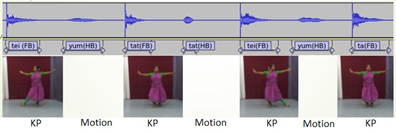
\includegraphics[scale= 1]{./Pictures/motion_fig.png}
  \caption{Occurrence of Motion and KPs}
  \label{fig:Ch1F004}
\end{figure}

There are various steps involved in Bharatanatyam dance. 
In Bharatanatyam, the dancer takes momentarily stationary well-defined posture, which occurs within each Adavus followed by sophisticated or complex motions frames. These are called Key Posture (KP).
Then, there are some frames associated with a Key Posture. They are called Key Frames.
During the dance, there is a transition from one Key Posture to the next Key Posture. They are called Motion (M). Motions (M) and Key Postures (KP) occur alternately and may repeat in a Bharatanatyam dance performance. Suppose there is Bharatanatyam dance Performance P, which consists of the interleaving sequence of Keyframes and motion frames like K1 M1 K2 M2 K3 M3 ... K(n-1) M(n-1) Kn. Where K is Keyframe, M is a motion frame,1,2,3...,n is $1^st$, $2^nd$, $3^rd$, ..., $n^th$ Keyframe or motion frame and n is the total frame. A motion comprised of several set of frames those are not momentarily stationary.






















\chapter{Literature Survey \& Problem Motivation} % Main chapter title

\label{Chapter 2} 
\lhead{Chapter 2. \emph{Literature Survey \& Problem Motivation}} 

In this chapter, we will discuss the literature survey, problem motivations and difficulty or challenges faced during project completion.


\section{Literature Survey}
Tanwi Mallick et al. develop NrityaGuru – an autonomous coaching system to give real-time instructional feedback regarding the accuracy of Bharatanatyam as performed by a learner.

Manel Sekma et al. proposes motion descriptor called Seg SIFT-ACC for human motion recognising. It is based on temporal segmentation into elementary motion segments. \citep{sekma2013human}

Matthew Cooper et al. presented approach on temporal video segmentation using supervised machine learning classification. So, we have also tried to use supervised machine learning in the given project.
They have created standard features through pairwise similarity of images. \citep{cooper2007video}

Rizwan Chaudhry et al. suggested a method for representing every frame of a video using a Histogram of oriented optical flow (HOOF). It is used for recognizing human actions by classifying HOOF time-series. \citep{chaudhry2009histograms}

Local histogram approaches used local spatiotemporal characteristics or feature for representing human activity in a video. \citep{laptev2005space}

Optical flow histograms were applied to match the movement(motion) of a player in a soccer match to that of a subject in a control video.  \citep{efros2003recognizing}

Tran et al. present an optical flow and shape-based approach that uses separate histograms for the horizontal and vertical components of the optical flow as well as the contour of the person as a motion descriptor. \citep{tran2008human}

Guozhu Liu at el. showed Key Frame Extraction method from compressed MPEG  video data. It helps in reducing Video processing time significantly.It helps in video segmentation and Keyframe extraction. \citep{liu2010key}.

Konečný, J. and Hagara, M used RGB, depth images and combine appearance (Histograms of Oriented Gradients) and motion descriptors (Histogram of optical flow) for parallel temporal segmentation and recognition. \citep{konevcny2014one}


\newpage
\section{Motivation}
Keyframe, motion frame and Key Posture detection is a fundamental step towards the analysis of dance steps in Bharatanatyam with the perspective of computer vision and human-computer interaction.
\begin{itemize}
    \item Distinguish Keyframe to motion frame can be used to automate or design an annotation tool. An annotation tool is used to determine which are Keyframe or motion frame 
    \item If the Keyframe is detected, we could recognize Adavu based on the occurrence of key-posture sequences. If the motion frame is detected, we could be able to classify the motion in the given Adavu.
\end{itemize}

Optical flow is the pattern of the apparent motion of objects, surfaces, and edges in a visual scene created by the relative motion between an observer and a scene \citep{wiki:003}. It is the distribution of ostensible(apparent) velocities of motion of illumination patterns in a scene or image \citep{wiki:003}.
\begin{itemize}
    \item Detection of Keyframe and motion frame from given set frames from Adavus video.
    \item Optical flow is used to extract the feature from the Gray frame of video as our main objective is to classify the motion frame and Keyframe from frames of video.
    \item Histogram of optical flow (HOOF) used as a final feature vector to input for binary the classifier.

\end{itemize}

\section{Challenges}
During the analysis of the keyframe and motion frame, some fundamental difficulties have been faced.

\begin{itemize}
    \item \textbf{Challenges 1}: At the start of the transition. There may be some very slow motions. That slow-motion may be falsely classified as Keyframe.
    
    \item \textbf{Challenges 2}: The distinction between Keyframe and motion frames may not be accessible due to the existence of complex motions and postures.
    
    \item \textbf{Challenges 3}: Non-visibility of foot/leg movements and occlusion due to the sophisticated dress style.
    
    \item \textbf{Challenges 4}: In some cases, when a dancer is in Key posture position, the movement of the dress materials may be misinterpreted as body movements( motion frame).
    
    \item \textbf{Challenges 5}: The non-availability of annotated Bharatanatyam Adavus.
\end{itemize} 
\chapter{Dataset Introduction} % Main chapter title

\label{Chapter 3} 
\lhead{Chapter 3. \emph{Dataset Introduction}} 

In this chapter, we will discuss the dataset and data analysis. 
Data set for Bharatanatyam Adavus is not open-sourced for research purpose.

\section{Dataset Introduction}
 So, We have recorded different dance formats for Adavus Bharatanatyam with the help of experts, dancers and learners. For the creation of dataset for Bharatanatyam adavus, Microsoft Kinect \cite{wiki:002} is used to capture RGB, skeleton videos and depth at a rate of 30 frames per second (fps).
 
\begin{figure}[hbt!]
  \centering
  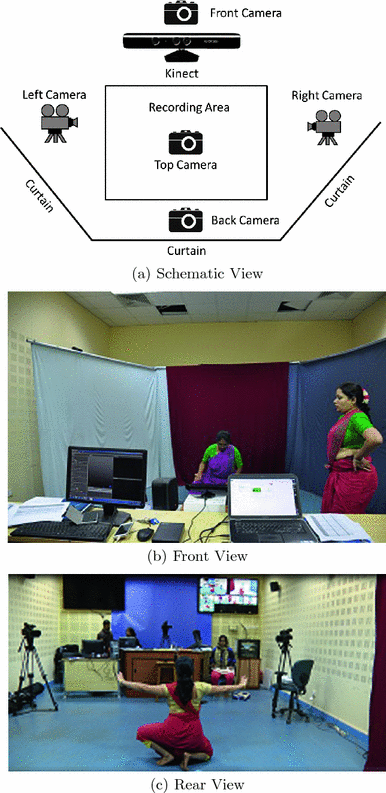
\includegraphics[scale= 0.5]{./Pictures/setup.png}
  \caption{Bharatanatyam Studio setup for recording}
  \label{fig:Ch03F001}
\end{figure}
The setup used for recording data set is shown in Figure \ref{fig:Ch03F001}

In this section of the project, only RGB frames are required for research purpose. Our approach was using a set of standard RGB as input and resized from 480 x 640 to 120 x 160 RGB frames, which had been further converted to grey frames for background subtraction.


The following Adavus had been recorded as a data set.
\begin{enumerate}
    \item Joining
    \item Kartari
    \item Nattal 
    \item Tattal 
    \item Mandi
    \item Mettu 
    \item Natta 
    \item Paikal
    \item Pakka
    \item Sarika 
    \item Sarikkal
    \item Tatta 
    \item Tei-Tei Dhatta
    \item Tirmana
    \item Utsanga
\end{enumerate}

\begin{table}[]
\hspace{-3cm}
\begin{tabular}{|c|c|c|c|c|c|c|}
\hline
\textbf{ADAVU} & \textbf{Variant} & \textbf{\# Dancers} & \textbf{\# Videos} & \textbf{\# Frames} & \textbf{\# Motion Frame} & \textbf{\# Key Frame} \\ \hline
\textbf{Tatta}          & 8  & 3 & 24  & 27155  & 12531 & 14624 \\ \hline
\textbf{Natta}          & 8  & 3 & 24  & 18587  & 9546  & 9041  \\ \hline
\textbf{Kuditta Mettu}  & 4  & 3 & 12  & 8895   & 4325  & 4570  \\ \hline
\textbf{Kuditta Nattal} & 6  & 3 & 18  & 15743  & 9816  & 5927  \\ \hline
\textbf{Kuditta Tattal} & 5  & 3 & 15  & 20995  & 13424 & 7571  \\ \hline
\textbf{Tei Tei Dhatta} & 3  & 3 & 9   & 5598   & 4336  & 1262  \\ \hline
\textbf{Katti Kartari}  & 1  & 3 & 3   & 2449   & 1747  & 702   \\ \hline
\textbf{Utsanga}        & 1  & 3 & 3   & 1363   & 1085  & 278   \\ \hline
\textbf{Mandi}          & 2  & 3 & 6   & 9975   & 5449  & 4526  \\ \hline
\textbf{Tirmana}        & 3  & 3 & 9   & 6415   & 4181  & 2234  \\ \hline
\textbf{Sarika}         & 4  & 3 & 12  & 8492   & 5662  & 2830  \\ \hline
\textbf{Joining}        & 3  & 2 & 6   & 4460   & 3110  & 1350  \\ \hline
\textbf{Total}          & 48 &   & 141 & 130127 & 75212 & 54915 \\ \hline
\end{tabular}
\caption{Bharatanatyam, Data set introduction}
\label{tab:Ch01T01}
\end{table}

Each Adavus have different numbers of variants. For each variation, three different dancers have performed Bharatanatyam dance. The data set has been shown in Table \ref{tab:Ch01T01}

After analyzing the dataset, we have observed that the annotation file for some of the Adavus and variation are not available. So, we have removed it from here as it is not relevant for us.

\begin{figure}[hbt!]
\centering
  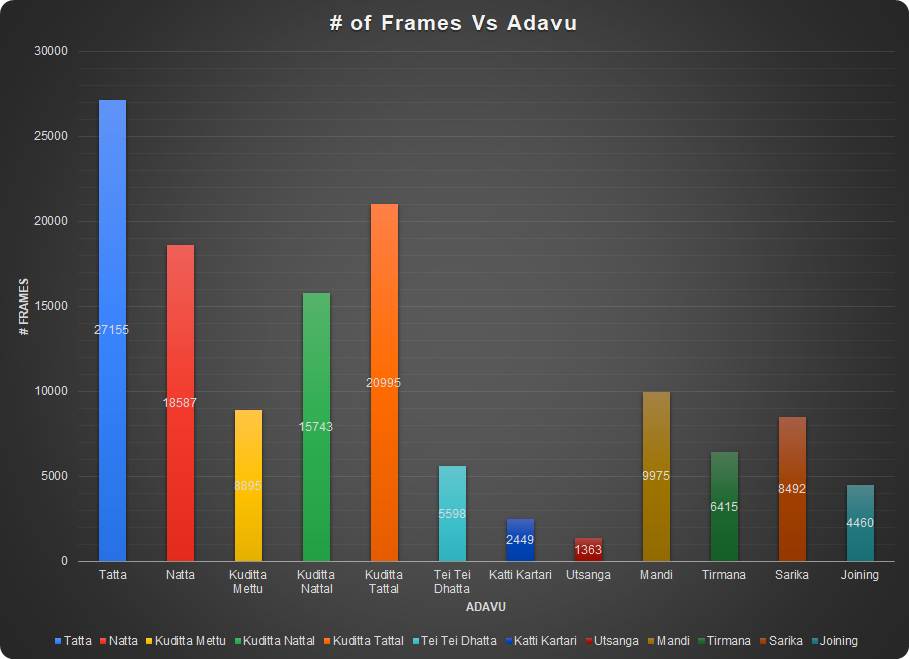
\includegraphics[scale= 0.8]{./Pictures/DataSet_Introduction.png}
  \caption{Bharatanatyam,Pictorial representation Data set}
  \label{fig:Ch03F002}
\end{figure}


\begin{table}[]
\centering
\begin{tabular}{|c|c|c|}
\hline
\textbf{ID}         & \textbf{Start Frame \#} & \textbf{End Frame \#} \\ \hline
\textbf{D1T4P01B1}  & 267                    & 303                  \\ \hline
\textbf{D1T4P01B2}  & 315                    & 350                  \\ \hline
\textbf{D1T4P01B3}  & 361                    & 396                  \\ \hline
\textbf{D1T4P01B4}  & 409                    & 444                  \\ \hline
\textbf{D1T4P01B5}  & 458                    & 494                  \\ \hline
\textbf{D1T4P01B6}  & 507                    & 542                  \\ \hline
\textbf{D1T4P01B7}  & 554                    & 590                  \\ \hline
\textbf{D1T4P01B8}  & 603                    & 643                  \\ \hline
\textbf{D1T4P01B9}  & 656                    & 684                  \\ \hline
\textbf{D1T4P01B10} & 697                    & 728                  \\ \hline
\textbf{D1T4P01B11} & 742                    & 775                  \\ \hline
\textbf{D1T4P01B12} & 788                    & 821                  \\ \hline
\textbf{D1T4P01B13} & 834                    & 865                  \\ \hline
\textbf{D1T4P01B14} & 879                    & 912                  \\ \hline
\textbf{D1T4P01B15} & 924                    & 953                  \\ \hline
\textbf{D1T4P01B16} & 966                    & 996                  \\ \hline
\end{tabular}
\caption{Tatta, Variant 4, Dancer 1 annotation file}
\label{tab:Ch01T02}
\end{table}


Each Adavu follows a regular pattern; for two consecutive Keyframe, there exist motion frames. All frames before 267, i.e., 1 to 265, are dancer preparing frame so that we would discard all frames. For example, in the first row, 267 is starting a Keyframe, and 303 is ending the Keyframe. After 303, i.e., from 304 to 314 are motion frames, and again Keyframe would be repeated similarly in Table.\ref{tab:Ch01T02}

\chapter{Workflow} % Main chapter title

\label{Chapter 4} 
\lhead{Chapter 4. \emph{Workflow}} 

In this chapter, we will discuss the workflow of our project and some algorithm.



\section{Workflow}
In this section, we will discuss the proposed workflow.
It takes RGB frame and outputs labelled feature as Keyfeature\textbf{(KF)} and motion frame \textbf{(MF)}. Classification of Keyfeature\textbf{(KF)} or non-motion frame and motion frame \textbf{(MF)} comprises the following parts:

\subsection{Background Subtraction Module}

\subsubsection{RGB image to Grayscale image:} 
It takes a colour image(RGB channels) of size 480 x 640. After that, the RGB image is converted to grayscale (single grayscale channel) of size 480 x 640. It helps in decreasing the complexity of the introduced method. Grayscale pixel’s value is computed by the weighted sum of the corresponding red, green, and blue pixels as:

\[\Large GrayFrame(i, j) = 0.299 \ast Frame(i, j)_R\]
\[\Large + 0.587 \ast Frame(i, j)_G\]
\[\Large + 0.144 \ast Frame(i, j)_B\]
\[\Large Where 1 \leqslant i \leqslant 480 and 1 \leqslant j \leqslant 640\]

\subsubsection{Background Removal}

\begin{figure}[H]
    \centering
    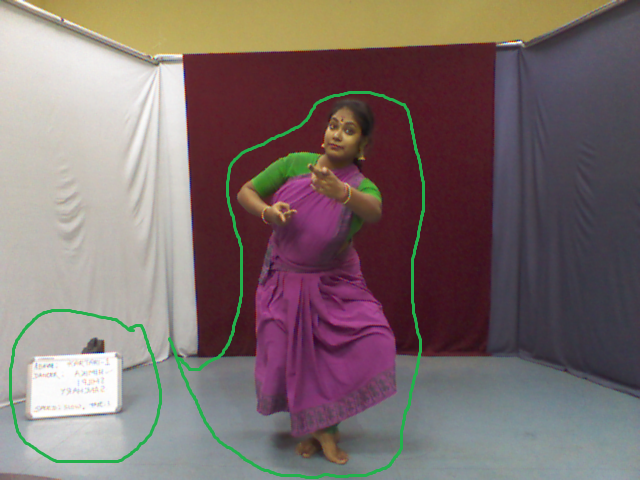
\includegraphics[scale= 0.7]{./Pictures/background_image.png}
    \caption{Redundant information highlighted}
    \label{fig:Ch04F001}
\end{figure}
Dancer image contains lots of redundant information which is not required for us—for example, background image or board on the side of the dancer, as shown in Figure \ref{fig:Ch04F001}. 

\begin{figure}[H]
\centering
  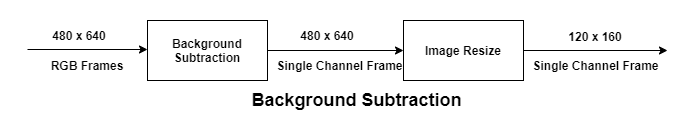
\includegraphics[scale= 0.6]{./Pictures/Algorithm-Background_Subtration.png}
  \caption{Background Subtraction}
  \label{fig:Ch04F002}
\end{figure}


Kinect depth data has 16-bit information, which consists of 3 bits which signify player index and the remaining 13 bits mean depth data. The depth data is the distance between the dancer and the camera lens. It uses the following algorithm as shown in Figure \ref{fig:Ch04F003}

\begin{figure}[H]
\centering
  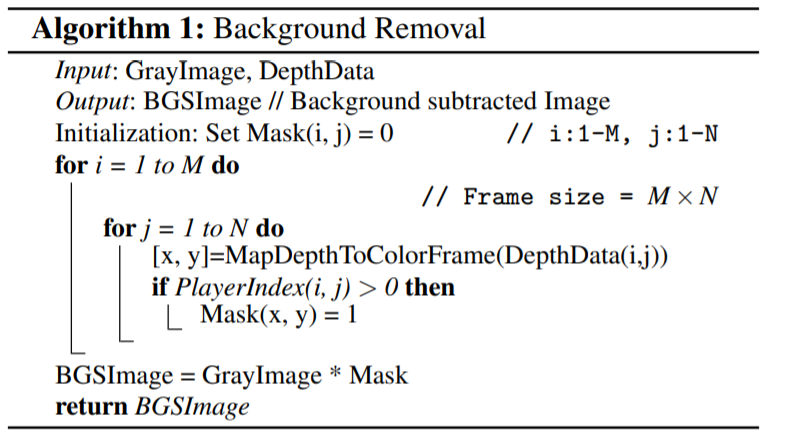
\includegraphics[scale= 0.7]{./Pictures/algo_image.png}
  \caption{Background Subtraction algorithm}
  \label{fig:Ch04F003}
\end{figure}

Since we are calculating optical flow which using motion information, so, we would remove the background from a grey image and retain only the information dancer portion. We would use depth stream information from Kinect depth
data as shown on Figure \ref{fig:Ch04F002} and \ref{fig:Ch04F003}.

\subsubsection{Resize Image}
After that, the image is resized to size $120 \ast 160$. We have used OpenCV, \texttt{\textbf{cv2.resize()}} function for this purpose. This function takes an image of size $480 \ast 640$ and resizes the image source down to size $120 \ast 160$, as shown in Figure \ref{fig:Ch04F002}
    





\subsection{Preprocessing Example (Backgroud Subtraction)}
\begin{figure}
    \centering
    \subfigure[]{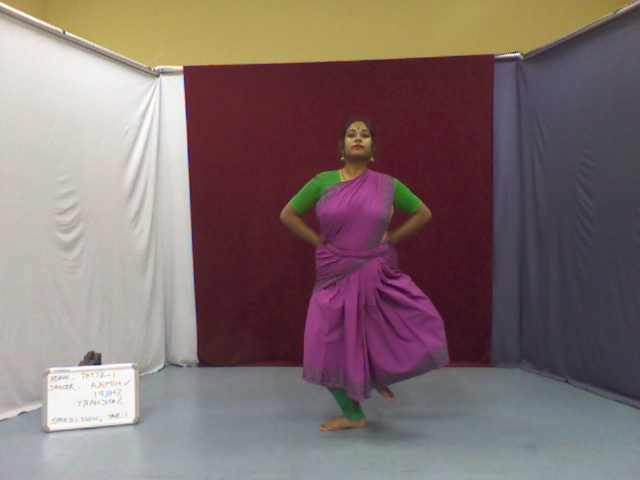
\includegraphics[width=0.22\textwidth]{Pictures/1_1.png}} 
    \subfigure[]{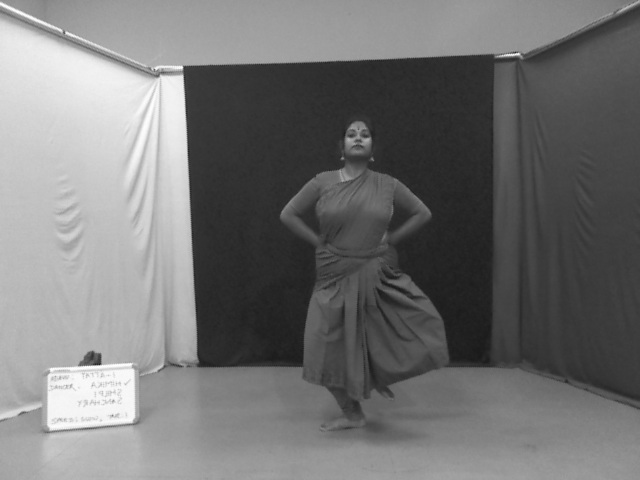
\includegraphics[width=0.22\textwidth]{Pictures/1_2.png}} 
    \subfigure[]{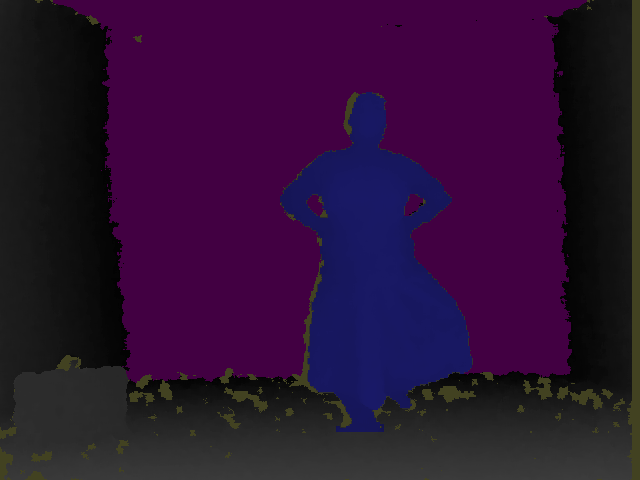
\includegraphics[width=0.22\textwidth]{Pictures/1_3.png}}
    \subfigure[]{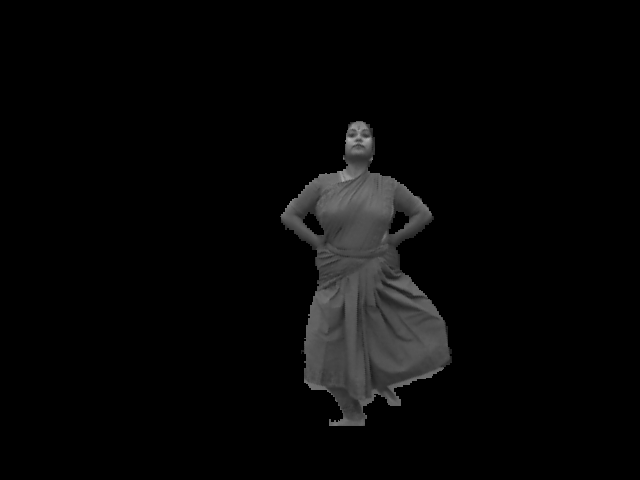
\includegraphics[width=0.22\textwidth]{Pictures/1_4.png}}
    \caption{(a) RGB (b) Grey (c) Depth Frame (d) Single channel}
    \caption{Tatta-$>$Variation-$>$Dancer 1}
    \label{fig:Ch04F004}
\end{figure}
 
\begin{figure}
    \centering
    \subfigure[]{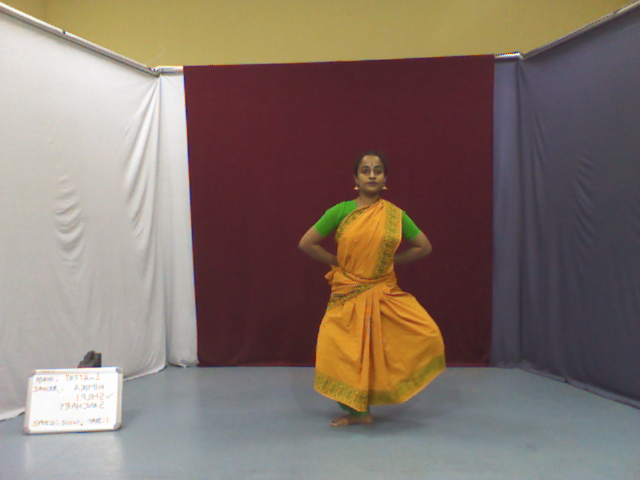
\includegraphics[width=0.22\textwidth]{Pictures/2_1.png}} 
    \subfigure[]{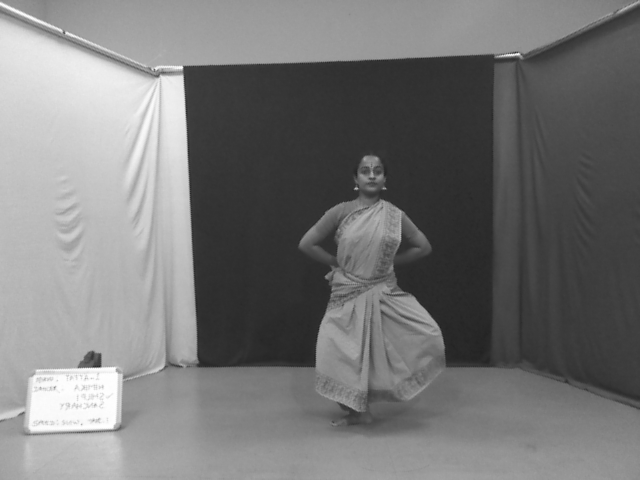
\includegraphics[width=0.22\textwidth]{Pictures/2_2.png}} 
    \subfigure[]{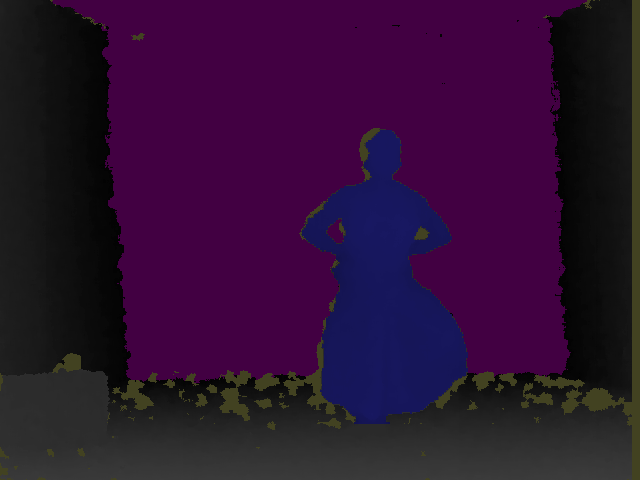
\includegraphics[width=0.22\textwidth]{Pictures/2_3.png}}
    \subfigure[]{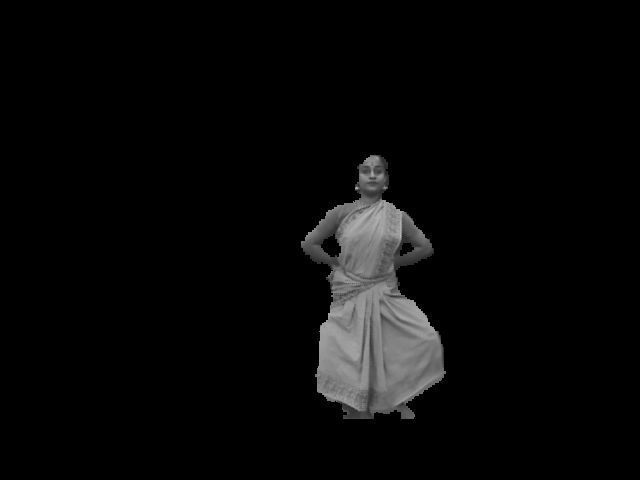
\includegraphics[width=0.22\textwidth]{Pictures/2_4.png}}
    \caption{(a) RGB (b) Grey (c) Depth Frame (d) Single channel}
    \caption{Tatta-$>$Variation-$>$Dancer 2}
    \label{fig:Ch04F005}
\end{figure}
 
 \begin{figure}
    \centering
    \subfigure[]{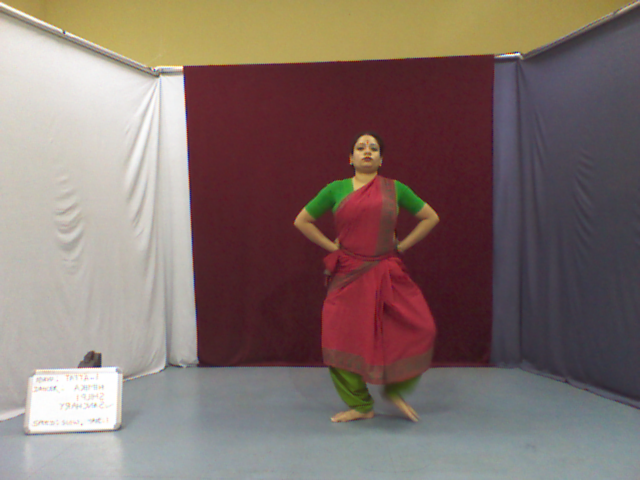
\includegraphics[width=0.22\textwidth]{Pictures/3_1.png}} 
    \subfigure[]{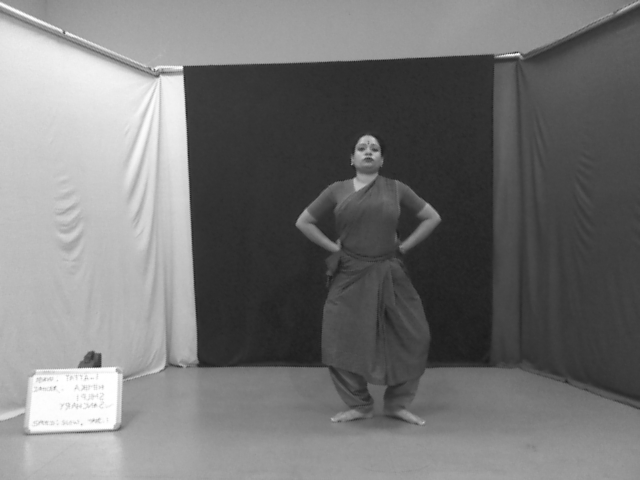
\includegraphics[width=0.22\textwidth]{Pictures/3_2.png}} 
    \subfigure[]{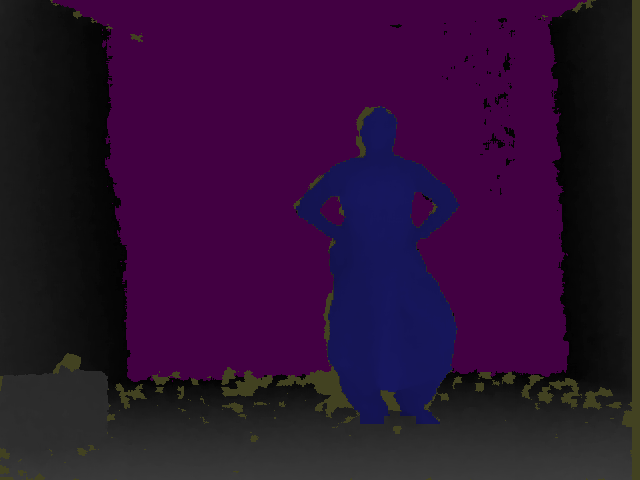
\includegraphics[width=0.22\textwidth]{Pictures/3_3.png}}
    \subfigure[]{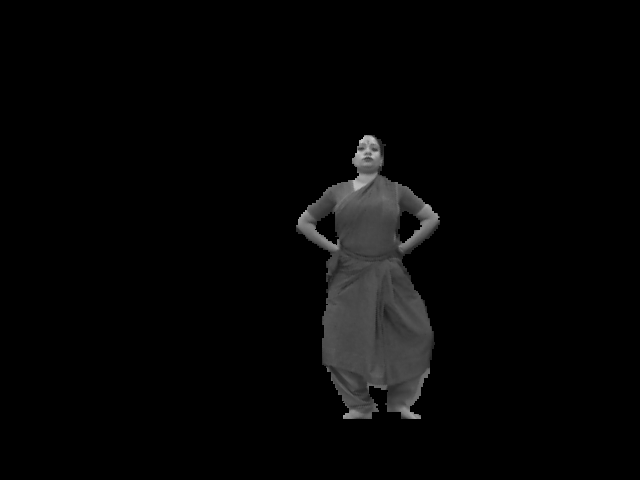
\includegraphics[width=0.22\textwidth]{Pictures/3_4.png}}
    \caption{(a) RGB (b) Grey (c) Depth Frame (d) Single channel}
    \caption{Tatta-$>$Variation-$>$Dancer 3}
    \label{fig:Ch04F006}
\end{figure}

It is the example of background removal as shown in Figure \ref{fig:Ch04F004}, \ref{fig:Ch04F005} and \ref{fig:Ch04F006}.
 
 
    
    
    
    
\subsection{Feature Extraction Module}

\begin{figure}[H]
  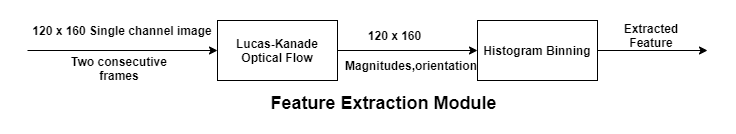
\includegraphics[scale= 0.5]{./Pictures/Algorithm-Feature_Extraction.png}
  \caption{Feature Extraction}
  \label{fig:Ch04F007}
\end{figure}
In this section, we will explain the feature extraction method used. This feature would be used for classification KeyFrame and motion frame (non-KeyFrame) in given Bharatnatyam adavu video. Lucas-Kanade optical flow is calculated. Two consecutive frames of size 120 x 160 single-channel images are taken as input. Lucas-Kanade optical flow method yield a matrix of size 120*160, which contains magnitudes and orientations. These are considered as input for Histogram binning. Histogram binning methods depend on the approaches we have taken. These would output the final feature vector for labelling. Different type of Histogram binning is used to feature descriptor.



    
\subsubsection{Estimate Optical Flow: Lucas-Kanade Method}


'opticalFlowLK' is used to estimate the optical flow using the Lucas-Kanade method \citep{barron1994performance}. This function generates an optical flow object for determining the direction(displacement) and speed of an apparent moving object using the Lucas-Kanade method(optical flow calculation method).

\begin{figure}
    \centering
    \subfigure[]{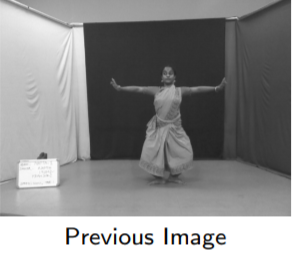
\includegraphics[width=0.32\textwidth]{Pictures/image1.png}} 
    \subfigure[]{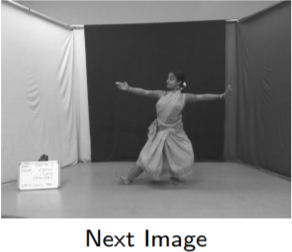
\includegraphics[width=0.32\textwidth]{Pictures/image2.png}} 
    \subfigure[]{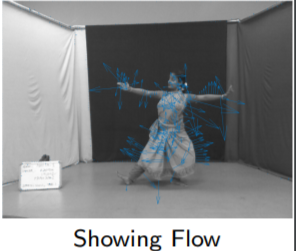
\includegraphics[width=0.32\textwidth]{Pictures/image3.png}} 
    \caption{(a) Previous Image (b) Next Image (c) Showing Image}
    \label{fig:Ch04007}
\end{figure}

\subsubsection{Algorithms}
\begin{enumerate}
    \item Input: Two consecutive images
    \item Output: Optical flow / velocity vector $(V_x, V_y) = (u, v)$ for each pixel
    \item Assumption: Brightness/ Intensity doesn’t change with time. So, $I(x, y, t) = I(x + u, y + v, t)$
\end{enumerate}

\begin{itemize}
    \item $I_x, I_y$, and It are the spatiotemporal image brightness derivatives.
    \item $u$ is the horizontal velocity vector.
    \item $v$ is the vertical velocity vector.
\end{itemize}
\[\huge I_xu+I_yv+I_t=0\]

\subsubsection{Lucas-Kanade Method}
The Optical flow constraint equation is solved using the Lucas-Kanade for $u$ \& $v$, the method splits the initial image into smaller segments and assumes a consistent velocity in each region.
A weighted and least-square fit is performed on the optical flow constraint equation to a consistent model for $[u  v]^T$ in each section of $\Omega$.
The given process achieves that fit by minimizing following the given equation:
\[\sum_{x \in Q} W^2 [I_xu + I_yv + I_t]^2\]

W is a window function for the center of each section. The solution to the minimization problem is:

\[\begin{bmatrix} & \sum W^2I_x^2 & \sum W^2I_xI_y \\
& \sum W^2I_yI_x & \sum W^2I_y^2 \end {bmatrix}\begin{bmatrix} & u\\ & v\end{bmatrix} = -\begin{bmatrix} & \sum W^2I_xI_t \\
& \sum W^2I_yI_t \end{bmatrix}\]


\subsubsection{Histogram Binning}
Histograms are utilized broadly as non-parametric frequency estimators for visualizing data and for obtaining extract quantities. However, the values of frequency estimators depend on the number of bins taken for the Histogram. There are some rules to determine bins number. For example, Generally, 5-20 bins numbers are satisfactory. As in the case of Matlab, ten(10) bins number is used as a default parameter.
We have used following Histogram binning method:

\begin{enumerate}
    \item Global Histogram using only magnitudes of optical flow.
    \item Global Histogram using magnitudes and orientation of optical flow.
    \item Fractional Histogram Binning using magnitudes and orientation of     optical flow taken over $8 \ast 8$ cell.
\end{enumerate}
    

\subsection{Training Module}
\begin{figure}[H]
    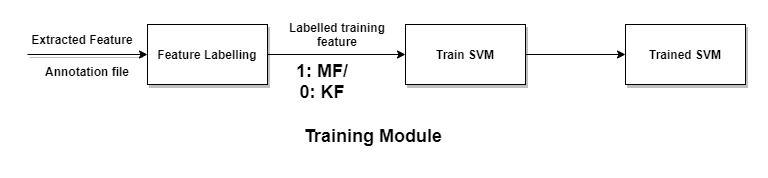
\includegraphics[scale= 0.6]{./Pictures/Algorithm-Training_Module.png}
    \caption{Training Module}
    \label{fig:Ch04F012}
\end{figure}
Extracted feature from the previous module with the help of annotation file is used to train the SVM classifier as shown in Figure \ref{fig:Ch04F012}.


\subsubsection{Feature Labeling}
Extracted feature and annotation file in ’CSV’ format is taken as input for feature labelling. The feature is marked as 1 for motion frame as this is our primary and as 0 for the KeyFrame as shown in Figure \ref{fig:Ch04F012}.



\subsubsection{Training SVM}
SVM(Support vector machine) is a mechanism of pattern identification that has a precise theoretical basis. So, we used a linear SVM classifier for feature labelling whether it is KeyFrame or motion frame.
Data set means a set of all motion frames and KeyFrame (non-motion frame).
The features are generated by Histogram binning in the previous section.
The dataset containing all frames was randomly separated into two datasets, i.e., training dataset and test dataset. The training dataset includes 80 per cent, both motion frames, and KeyFrames. Test dataset contains 20 per cent also contain both motion frames and KeyFrames.



\begin{lstlisting}
kernel = 'linear'
#Create a svm Classifier
clf = svm.SVC(kernel=kernel)  # Linear Kernel

#Train the model using the training sets
clf.fit(X_train, y_train)
\end{lstlisting}


    
    
 \subsection{Testing Module}
We would use the test dataset, i.e., the test feature vector is used on trained SVM. This trained SVM would label a given frame, whether it is motion frame(MF:1) or KeyFrame (KF:0) as shown in Figure \ref{fig:Ch04F013}.

 \begin{figure}[H]
  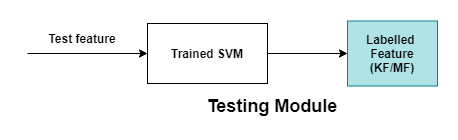
\includegraphics[scale= 0.7]{./Pictures/Algorithm-Testing_Module.png}
  \caption{Testing Module}
  \label{fig:Ch04F013}
\end{figure}
 
 \subsubsection{Evaluation metrics}
Some motion frames will be detected as KeyFrame and some KeyFrame will be detected as motion frame.

We have used four usually accepted criteria, i.e.,
\begin{enumerate}
    \item Accuracy
    \item Precision
    \item Recall
    \item F1-Score
\end{enumerate}
It is used for the evaluation of prediction performance of constructed SVM binary classifier models. The accuracy is the number of correctly predicted KeyFrame and motion frame out of the total number of given frames. The precision is the number of actual KeyFrame and motion frame out of predicted KeyFrame and motion frame.
The recall is the number of correctly predicted KeyFrame and motion frame out of actual KeyFrame and motion frame
The F1 score value is a merged value of recall and precision.



\textbf{\[F1Score = 2* \frac{Precision * Recall}{Precisin + Recall} \]}

KeyFrame accuracy is determined by following formula:
\[Accuracy_{KF} = \frac{KF_{Detected}}{KF_{Total}}\]
where $Accuracy_{KF}$ : Accuracy of KeyFrame,\newline 
$KF_{Detected}$ : Number of detected KeyFrame \& \newline
$KF_{Total}$ : Total Number of KeyFrame.\newline

\[Accuracy_{MF} = \frac{MF_{Detected}}{MF_{Total}}\]
where $Accuracy_{MF}$ : Accuracy of Motion Frame,\newline 
$MF_{Detected}$ : Number of detected Motion Frame \& \newline
$MF_{Total}$ : Total Number of Motion Frame.\newline

No doubt we have computed for both motion frame(MF) and KeyFrame(KF). Our objective is to detect motion key(MF).

True Positive(TP) = Motion Frame
True Negative(TN) = Key Frame

\textbf{TP} = Motion frame when it was Motion frame.\newline
\textbf{TN} = Key frame when it was Key frame.\newline
\textbf{FP} = Motion frame when it was Key frame.\newline
\textbf{TN} = Key frame when it was Motion frame.\newline

\[
Accuracy_{Total} = \frac{KF_{Correct\_Detected} + MF_{Correct\_Detected}}{KF_{Total} + MF_{Total}}
\]

\chapter{Histogram Binning} % Main chapter title

\label{Chapter 5} 
\lhead{Chapter 5. \emph{Histogram Binning}} 

In this chapter, we will discuss various histogram used in project.


\section{Histogram Binning}
The Histogram is a primary analytical tool for information analysis, which is accepted as an essential part of various experimental computational algorithms \citep{shams2007efficient}. In this section, we analyze multiple approaches used for the creation of a feature vector, as shown in the Figure\ref{fig:Ch05F001}.

 \begin{figure}[H]
  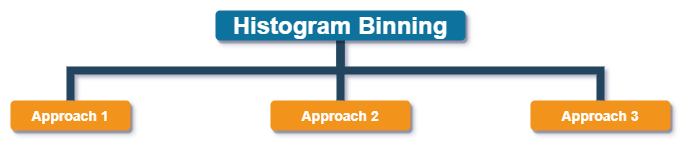
\includegraphics[scale= 0.5]{./Pictures/histogram_binning.png}
  \caption{Testing Module}
  \label{fig:Ch05F001}
\end{figure}




\subsection{Approach 1: Global Histogram using only magnitudes of optical flow}
In this section, we would discuss a global Histogram using only magnitudes of the optical flow of two consecutive images.
We are taking magnitudes part only of optical flow. Since our image size was \[120 \ast 160\], our input would be of size $19200$. We would sort the vector X into bins with intervals defined by the vector $numBins$ (Number of bins). Finally, it would output the frequency of elements in each bin. It would be returned as a feature row vector of size $9$.
The sample feature vector for two input images is the following:

\[[18611 ,173 ,142 ,115 ,71 ,50 ,29 ,4 ,5] \]



\subsection{Approach 2: Global Histogram using magnitudes and Orientation of optical flow}
In this section, we would discuss global histogram using magnitudes and Orientation of the optical flow of two consecutive images.

We are taking magnitudes and Orientation of optical flow. Since our image size was $120 \ast 160$, our input would be two matrices of size $120 \ast 160$.We would convert $120 \ast 160$ matrices to $19200$ vectors and calculation would be done.

It would create a Histogram of optical flow (HOOF) of the images, based on the respective weightage of magnitude with respect to orientations.
 Finally, it would output the frequency of elements in each bin. It would be returned as a feature row vector of size $9$.
 
 Sample feature vector for two input images is following:
\[[68.98, 5.93, 0, 0, 0, 0, 0, 0,21.13]\]





\subsection{Approach 3: Fractional Histogram Binning using  magnitudes and Orientation of optical flow taken over 8 x 8 cell}

In this section, we would discuss fractional Histogram using magnitudes and orientation of the optical flow of two consecutive images.
In this approach, we compute a HOOF descriptor vector for the supplied optical flow of two consecutive images.

We are taking magnitudes and orientation of optical flow. Since our image size was $120 \ast 160$, our input would be two matrices of size $120 \ast 160$. It would compute a local histogram of optical flow (HOOF) of $8 \ast 8$ pixel cells and concatenate to form a $9576$ feature vector.

The block size of $2 \ast 2$ cells is taken. There would be $9$ bins for each cell, \newline
so 
\[9 \ast 4 = 36\]
feature vector for a block. There would be a $50\%$ overlap between blocks. So that $15$ iterations over the vertical cell and $20$ repetitions over the horizontal cell.

\[{Feature\_Vector}_{\textbf{Total}} = (15 - 1) \ast (20 - 1 ) \ast 4 \ast 9 = 9576\]

It would be returned as a feature row vector of size 9.

 
 Sample feature vector of size $9576$ for two input images is following:
 
\[[0.004,0.002,0.543,0,0,...,0.003,0.006]\]
 

\chapter{Experimental Result} % Main chapter title

\label{Chapter 6} 
\lhead{Chapter 6. \emph{Experimental Result}} 

In this chapter, we would discuss various result.

\section{Global Histogram using only magnitudes of optical flow}
In this section, we would discuss the experimental result for Global Histogram using only magnitudes of optical flow. Since we have used only the magnitude part, there is poor accuracy.
There is a lot of information loss through orientation flow part.

\begin{table}[]
\centering
\hspace*{-2.5cm}
\begin{tabular}{|l|l|l|l|l|l|l|l|l|l|}
\hline
\textbf{Evaluation} &
  \multicolumn{3}{c|}{\textbf{Accuracy}} &
  \multicolumn{2}{c|}{\textbf{Precision}} &
  \multicolumn{2}{c|}{\textbf{Recall}} &
  \multicolumn{2}{c|}{\textbf{F1}} \\ \hline
Adavus         & MF + KF & MF    & KF    & MF    & KF    & MF    & KF    & MF    & KF    \\ \hline
Tatta          & 52.1    & 66.48 & 45.78 & 35.01 & 75.66 & 66.48 & 45.78 & 45.86 & 57.04 \\ \hline
Natta          & 59.26   & 64.3  & 55.32 & 52.92 & 66.49 & 64.3  & 55.32 & 58.06 & 60.39 \\ \hline
Kuditta Mettu  & 71.07   & 62.24 & 77.19 & 65.45 & 74.66 & 62.24 & 77.19 & 63.81 & 75.9  \\ \hline
Kuditta Nattal & 67.73   & 62.67 & 74.47 & 76.54 & 60.01 & 62.67 & 74.47 & 68.91 & 66.46 \\ \hline
Kuditta Tattal & 54.72   & 44.95 & 69.16 & 68.3  & 45.93 & 44.95 & 69.16 & 54.22 & 55.2  \\ \hline
Tei Tei Dhatta & 54.19   & 45.51 & 77.69 & 84.66 & 34.51 & 45.51 & 77.69 & 59.2  & 47.79 \\ \hline
Katti Kartari  & 68.88   & 63.04 & 80    & 85.71 & 53.2  & 63.04 & 80    & 72.65 & 63.91 \\ \hline
Utsanga        & 45.79   & 37.04 & 67.27 & 73.53 & 30.33 & 37.04 & 67.27 & 49.26 & 41.81 \\ \hline
Mandi          & 72.75   & 67.04 & 78.98 & 77.67 & 68.72 & 67.04 & 78.98 & 71.97 & 73.49 \\ \hline
Tirmana        & 48.51   & 35.45 & 69.82 & 65.71 & 39.87 & 35.45 & 69.82 & 46.06 & 50.75 \\ \hline
Sarika         & 47.81   & 33.91 & 70.39 & 65.06 & 39.58 & 33.91 & 70.39 & 44.59 & 50.67 \\ \hline
Joining        & 65.79   & 62.11 & 71    & 75.16 & 57.01 & 62.11 & 71    & 68.01 & 63.25 \\ \hline
\end{tabular}
\caption{Used only magnitudes for binning}
\label{tab:Ch06T001}
\end{table}


\begin{figure}[H]
    \hspace{-2.5cm}
    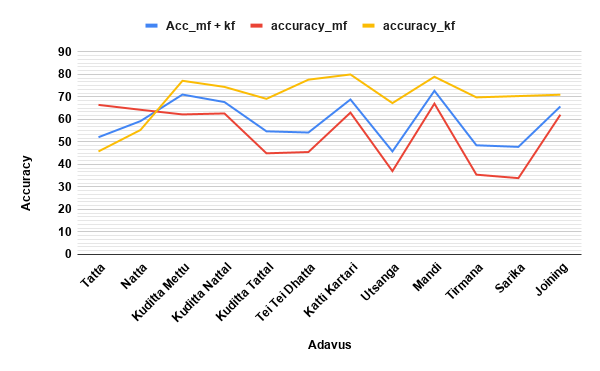
\includegraphics[scale= 0.8]{./Pictures/hist.png}
    \caption{Testing Module}
    \label{fig:Ch06F001}
\end{figure}

From the plot, we can see that accuracy for Keyframe is always higher than the accuracy of the motion frame except for two cases of Tatta and Natta.
Accuracy for motion frame and Keyframe combined lies between accuracy for Keyframe and motion frame except for two cases of Tatta and Natta. It is mainly due to the simple motion frame structure as compared to Keyframe in Tattaand Natta.



\section{Global Histogram using  magnitudes and Orientation of optical flow}
In this section, we would discuss the experimental result for global Histogram using magnitudes and orientation of optical flow since we have used the magnitude and orientation of optical flow. There should be better accuracy than better accuracy.
We have more information from the orientation of optical flow


\begin{table}[]
\centering
\hspace*{-1cm}
\begin{tabular}{|l|l|l|l|l|l|l|l|l|l|}
\hline
\multicolumn{1}{|c|}{\textbf{Evaluation}} &
  \multicolumn{3}{c|}{\textbf{Accuracy}} &
  \multicolumn{2}{c|}{\textbf{Precision}} &
  \multicolumn{2}{c|}{\textbf{Recall}} &
  \multicolumn{1}{c|}{\textbf{F1}} &
  \multicolumn{1}{c|}{\textbf{F1}} \\ \hline
\multicolumn{1}{|c|}{\textbf{Adavus}} &
  \multicolumn{1}{c|}{\textbf{MF + KF}} &
  \multicolumn{1}{c|}{\textbf{MF}} &
  \multicolumn{1}{c|}{\textbf{KF}} &
  \multicolumn{1}{c|}{\textbf{MF}} &
  \multicolumn{1}{c|}{\textbf{KF}} &
  \multicolumn{1}{c|}{\textbf{MF}} &
  \multicolumn{1}{c|}{\textbf{KF}} &
  \multicolumn{1}{c|}{\textbf{MF}} &
  \multicolumn{1}{c|}{\textbf{KF}} \\ \hline
Tatta          & 73.07 & 64.38 & 76.89 & 55.04 & 83.09 & 64.38 & 76.89 & 59.34 & 79.87 \\ \hline
Natta          & 73.79 & 67.28 & 78.88 & 71.33 & 75.53 & 67.28 & 78.88 & 69.25 & 77.17 \\ \hline
Kuditta Mettu  & 82.72 & 74.41 & 88.49 & 81.77 & 83.28 & 74.41 & 88.49 & 77.92 & 85.81 \\ \hline
Kuditta Nattal & 76.73 & 72.3  & 82.61 & 84.68 & 69.18 & 72.3  & 82.61 & 78    & 75.3  \\ \hline
Kuditta Tattal & 67.55 & 60.2  & 78.42 & 80.49 & 57.13 & 60.2  & 78.42 & 68.88 & 66.1  \\ \hline
Tei Tei Dhatta & 64.09 & 57.88 & 80.88 & 89.12 & 41.51 & 57.88 & 80.88 & 70.18 & 54.86 \\ \hline
Katti Kartari  & 70.66 & 64.59 & 82.22 & 87.37 & 54.95 & 64.59 & 82.22 & 74.27 & 65.88 \\ \hline
Utsanga        & 59.47 & 57.04 & 65.45 & 80.21 & 38.3  & 57.04 & 65.45 & 66.67 & 48.32 \\ \hline
Mandi          & 80.05 & 76.17 & 84.29 & 84.1  & 76.43 & 76.17 & 84.29 & 79.94 & 80.17 \\ \hline
Tirmana        & 61.21 & 53.53 & 73.73 & 76.88 & 49.31 & 53.53 & 73.73 & 63.11 & 59.1  \\ \hline
Sarika         & 51.18 & 35.55 & 76.6  & 71.18 & 42.23 & 35.55 & 76.6  & 47.42 & 54.44 \\ \hline
Joining        & 71.49 & 68.68 & 75.46 & 79.82 & 63.04 & 68.68 & 75.46 & 73.83 & 68.7  \\ \hline
\end{tabular}
\caption{Used magnitudes and Orientation for binning}
\label{tab:Ch06T002}
\end{table}








\begin{figure}[H]
    \hspace{-2.5cm}
    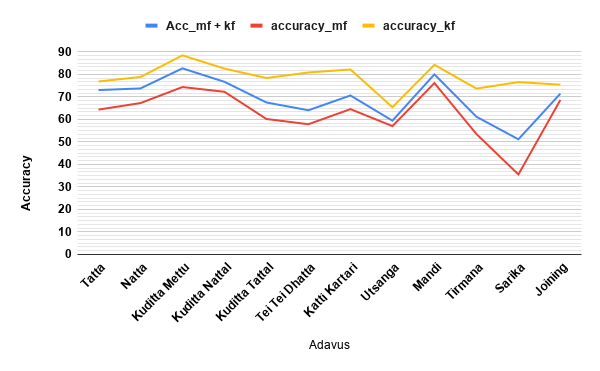
\includegraphics[scale= 0.8]{./Pictures/global.png}
    \caption{Testing Module}
    \label{fig:Ch06F002}
\end{figure}


\section{Fractional Histogram Binning using  magnitudes and Orientation of optical flow taken over 8 x 8 cell}



\begin{table}[]
\hspace*{-1.25cm}
\begin{tabular}{|l|l|l|l|l|l|l|l|l|l|}
\hline
Evaluation & \multicolumn{3}{l|}{Accuracy} & \multicolumn{2}{l|}{Precision} & \multicolumn{2}{l|}{Recall} & F1 & F1 \\ \hline
Adavus         & MF + KF & MF    & KF    & MF    & KF    & MF    & KF    & MF    & KF    \\ \hline
Tatta          & 87.76   & 73.63 & 93.96 & 84.27 & 89.03 & 73.63 & 93.96 & 78.59 & 91.43 \\ \hline
Natta          & 79.83   & 71.75 & 86.14 & 80.17 & 79.61 & 71.75 & 86.14 & 75.73 & 82.75 \\ \hline
Kuditta Mettu  & 81.04   & 69.98 & 88.71 & 81.14 & 80.98 & 69.98 & 88.71 & 75.15 & 84.67 \\ \hline
Kuditta Nattal & 77.2    & 82.61 & 70.15 & 78.29 & 75.59 & 82.61 & 70.15 & 80.39 & 72.77 \\ \hline
Kuditta Tattal & 77.5    & 70.2  & 88.42 & 90.49 & 67.13 & 70.2  & 88.42 & 78.88 & 76.1  \\ \hline
Tei Tei Dhatta & 81.08   & 88.66 & 60.56 & 85.88 & 66.38 & 88.66 & 60.56 & 87.25 & 63.33 \\ \hline
Katti Kartari  & 82.65   & 88.33 & 71.85 & 85.66 & 76.38 & 88.33 & 71.85 & 86.97 & 74.05 \\ \hline
Utsanga        & 78.95   & 85.19 & 63.64 & 85.19 & 63.64 & 85.19 & 63.64 & 85.19 & 63.64 \\ \hline
Mandi          & 80.59   & 85.26 & 73.98 & 82.23 & 78.04 & 85.26 & 73.98 & 83.72 & 75.95 \\ \hline
Tirmana        & 77.39   & 82.37 & 69.06 & 81.66 & 70.07 & 82.37 & 69.06 & 82.01 & 69.57 \\ \hline
Sarika         & 70.36   & 69.9  & 71.1  & 79.73 & 59.23 & 69.9  & 71.1  & 74.49 & 64.63 \\ \hline
Joining        & 80.59   & 85.26 & 73.98 & 82.23 & 78.04 & 85.26 & 73.98 & 83.72 & 75.95 \\ \hline
\end{tabular}
\caption{result: fractional histogram binning}
\label{tab:Ch06T003}
\end{table}



















\begin{figure}[H]
    % \centering
    \hspace{-2.5cm}
    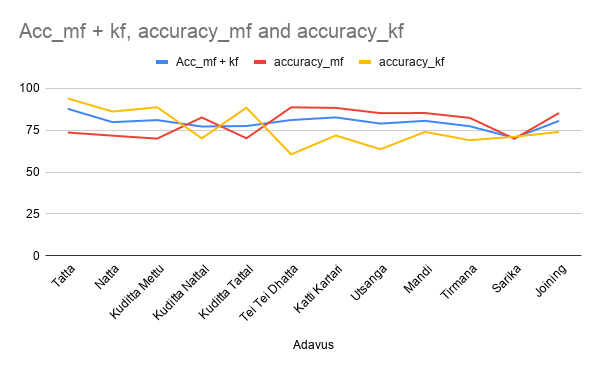
\includegraphics[scale= 0.8]{./Pictures/local.png}
    \caption{Testing Module}
    \label{fig:Ch06F003}
\end{figure}





\section{Comparison among different histogram approaches}






\begin{table}[]
\hspace{-2.5cm}
\begin{tabular}{|c|c|c|c|c|c|c|}
\hline
Approach       & Approach 1 & Approach 2 & Approach 3 & Approach 1 & Approach 2 & Approach 3 \\ \hline
Adavus         & \multicolumn{3}{c|}{MF}              & \multicolumn{3}{c|}{KF}              \\ \hline
Tatta          & 66.48      & 64.38      & 73.63      & 45.78      & 76.89      & 93.96      \\ \hline
Natta          & 64.30      & 67.28      & 71.75      & 55.32      & 78.88      & 86.14      \\ \hline
Kuditta Mettu  & 62.24      & 74.41      & 69.98      & 77.19      & 88.49      & 88.71      \\ \hline
Kuditta Nattal & 62.67      & 72.30      & 82.61      & 74.47      & 82.61      & 70.15      \\ \hline
Kuditta Tattal & 44.95      & 60.20      & 70.20      & 69.16      & 78.42      & 88.42      \\ \hline
Tei Tei Dhatta & 45.51      & 57.88      & 88.66      & 77.69      & 80.88      & 60.56      \\ \hline
Katti Kartari  & 63.04      & 64.59      & 88.33      & 80.00      & 82.22      & 71.85      \\ \hline
Utsanga        & 37.04      & 57.04      & 85.19      & 67.27      & 65.45      & 63.64      \\ \hline
Mandi          & 67.04      & 76.17      & 85.26      & 78.98      & 84.29      & 73.98      \\ \hline
Tirmana        & 35.45      & 53.53      & 82.37      & 69.82      & 73.73      & 69.06      \\ \hline
Sarika         & 33.91      & 35.55      & 69.90      & 70.39      & 76.60      & 71.10      \\ \hline
Joining        & 62.11      & 68.68      & 85.26      & 71.00      & 75.46      & 73.98      \\ \hline
\end{tabular}
\caption{Comparision between various approaches}
\label{tab:Ch06T004}
\end{table}











\begin{figure}[H]
    % \centering
    \hspace{-2.5cm}
    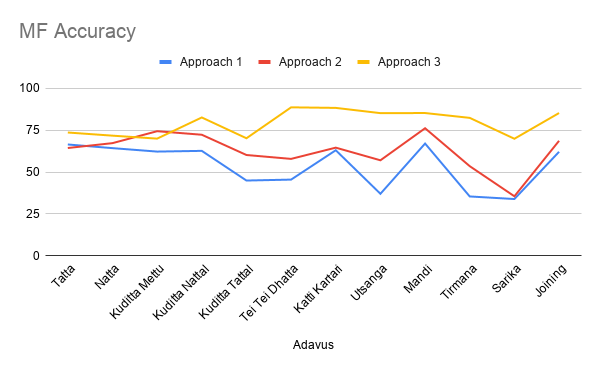
\includegraphics[scale= 0.8]{./Pictures/mf.png}
    \caption{Testing Module}
    \label{fig:Ch06F004}
\end{figure}

\begin{figure}[H]
    % \centering
    \hspace{-2.5cm}
    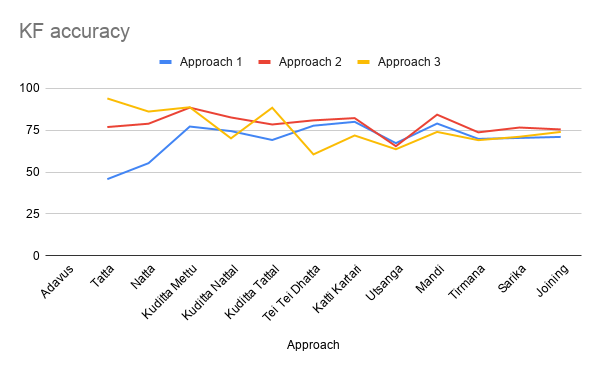
\includegraphics[scale= 0.8]{./Pictures/kf.png}
    \caption{Testing Module}
    \label{fig:Ch06F005}
\end{figure}





\section{Minimum accuracy plot}
    % \centering
    \begin{figure}[H]
    \hspace{-2.5cm}    
    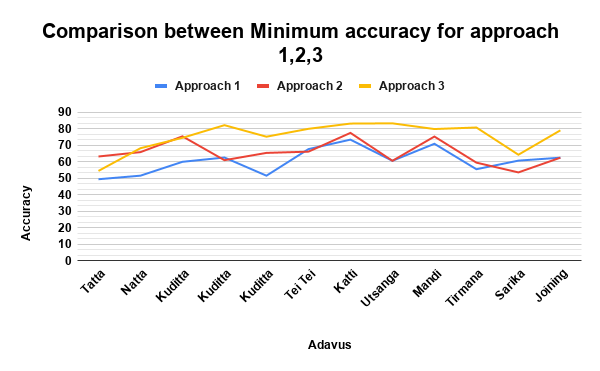
\includegraphics[scale= 0.8]{./Pictures/min.png}
    \caption{Minimum accuracy plot}
    \label{fig:Ch06F006}
\end{figure}

\section{Maximum accuracy plot}
    % \centering
    \begin{figure}[H]
    \hspace{-2.5cm}
    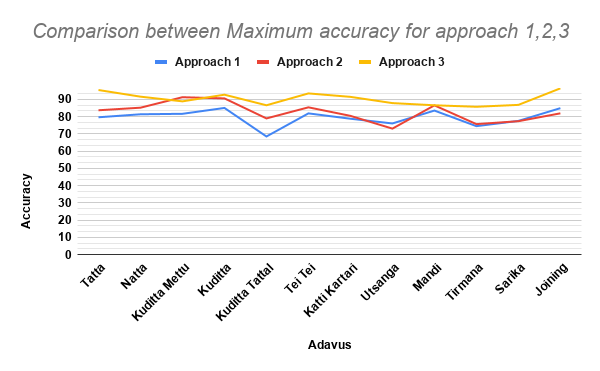
\includegraphics[scale= 0.8]{./Pictures/max.png}
    \caption{Maximum accuracy plot}
    \label{fig:Ch06F007}
\end{figure}

\chapter{Conclusion} % Main chapter title

\label{Chapter 7} 
\lhead{Chapter 7. \emph{Conclusion}} 

\section{Conclusion}
The proposed approach could successfully detect Keyframe and motion frame from given set frames from Adavus video. Optical flow help in the extraction of the feature.

Histogram of optical flow (HOOF) and histogram binning successfully helps in feature vector extraction. It is used as a final feature vector to train the binary SVM classifier.
Approach $3$ gives the best accuracy among all approaches because we are covering the whole image by block by block. It helps in the preservation of information and optical flow of the image.

\chapter{Acknowledgement} % Main chapter title

\label{Chapter 8} 
\lhead{Chapter 8. \emph{Acknowledgement}} 

\section{Acknowledgement}

This project authors fully acknowledge the support from Prof. Partha Pratim Das, Head, Rajendra Mishra School of Engineering Entrepreneurship, and Ph.D. student Himadri B.G.S. Bhuyan. We have taken immense help from MatLab software and its support community.

%----------------------------------------------------------------------------------------
%	THESIS CONTENT - APPENDICES
%----------------------------------------------------------------------------------------

\addtocontents{toc}{\vspace{2em}} % Add a gap in the Contents, for aesthetics

\appendix % Cue to tell LaTeX that the following 'chapters' are Appendices
\addtocontents{toc}{} % Add a gap in the Contents, for aesthetics

\backmatter

%----------------------------------------------------------------------------------------
%	BIBLIOGRAPHY
%----------------------------------------------------------------------------------------
\makeatletter
\renewcommand*{\@biblabel}[1]{\hfill#1.}
\makeatother

\nocite{*}
\label{Bibliography}

\medskip

\bibliographystyle{plainnat}
\bibliography{Bibliography}

\end{document}  
